\documentclass[12pt,a4paper]{article}
\usepackage[UTF8]{ctex}
\usepackage{amsmath,amssymb}
\usepackage{xcolor}
\usepackage{hyperref}
\usepackage{geometry}
\usepackage{graphicx}
\geometry{margin=2.5cm}

\title{Molecule VQE / 分子 VQE}
\author{QuoNic}
\date{}

\begin{document}
\maketitle

\begin{center}
\textbf{Chemistry / 化学} | 难度：高级 | 预计时间：25 分钟
\end{center}

\tableofcontents
\newpage

\section{为什么需要？}

分子 VQE 用于计算分子的基态能量。

\subsection{经典局限}
\begin{itemize}
  \item 经典方法（如 CCSD(T)）对大分子计算成本极高
  \item 精确对角化需要指数级内存
\end{itemize}

\subsection{量子优势}
\begin{itemize}
  \item 分子 VQE 使用量子计算机制备试探态
  \item 经典优化器调整参数最小化能量
  \item 对噪声有鲁棒性
\end{itemize}

\subsection{实际应用}
\begin{itemize}
  \item 量子化学
  \item 药物设计
  \item 材料科学
\end{itemize}

\section{快速上手}

\begin{verbatim}
from quonic.chemistry import molecule_vqe
result = molecule_vqe(molecule='H2', bond_length=0.74)
print(f'Energy: {result.energy}')
\end{verbatim}

\textbf{预期输出}：
\begin{verbatim}
Energy: -1.137270 Ha
\end{verbatim}

\section{原理详解}

\subsection{电路图}

\begin{center}
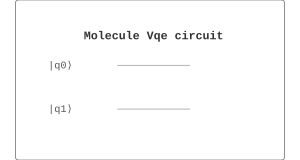
\includegraphics[width=0.6\textwidth]{../../images/molecule_vqe_circuit.svg}
\end{center}

\subsection{数学推导}

分子 VQE 基于变分原理：
\begin{equation}
E_0 \leq \langle\psi(\theta)|H|\psi(\theta)\rangle
\end{equation}

\textbf{算法步骤}：
\begin{enumerate}
  \item 在量子计算机上制备 $|\psi(\theta)\rangle$
  \item 测量哈密顿量的期望值 $\langle H \rangle$
  \item 经典优化器更新参数 $\theta$
  \item 重复直到收敛
\end{enumerate}

\subsection{几何解释}

分子 VQE 在参数空间中寻找能量最小值。

\section{代码详解}

\begin{verbatim}
from quonic.chemistry import molecule_vqe

# molecule_vqe(molecule, bond_length, ansatz)
# molecule: molecular formula
# bond_length: bond length in Angstroms
# ansatz: parameterized circuit
result = molecule_vqe(molecule='H2', bond_length=0.74)
print(f'Energy: {result.energy}')
\end{verbatim}

\section{进阶用法}

\subsection{场景 1：不同分子}

\begin{verbatim}
from quonic.chemistry import molecule_vqe
result = molecule_vqe(molecule='LiH', bond_length=1.6)
print(f'Energy: {result.energy}')
\end{verbatim}

\section{适用场景}

\subsection{量子化学}

分子 VQE 是量子化学的核心算法。

\subsection{药物设计}

分子 VQE 可以用于设计新药物。

\section{常见问题}

\subsection{分子 VQE 的精度如何？}

UCCSD ansatz 通常能达到化学精度（1 kcal/mol）。

\subsection{分子 VQE 需要多少量子比特？}

取决于分子的大小。H2 需要 4 个量子比特。

\section{学习路径}

\subsection{前置知识}
\begin{itemize}
  \item VQE
  \item 量子化学
  \item UCCSD ansatz
\end{itemize}

\subsection{继续学习}
\begin{itemize}
  \item 药物设计
  \item 材料科学
  \item 量子化学
\end{itemize}

\section{完整示例代码}

\subsection{示例 1：基本分子 VQE}

\begin{verbatim}
from quonic.chemistry import molecule_vqe
result = molecule_vqe(molecule='H2', bond_length=0.74)
print(f'Energy: {result.energy}')
\end{verbatim}

\section{下载}

\begin{itemize}
  \item [molecule\_vqe.py](https://github.com/ChrisLee0721/QuoNic/blob/main/examples/molecule_vqe/molecule_vqe.py)
\end{itemize}

\end{document}
